\chapter{Programming Assignment 3}

\begin{marginfigure}
  \begin{center}
    \includegraphics[width=\textwidth]{Assignments/figures/nsf_ligo.jpg}
  \end{center}
  \caption{Artist's depiction of gravitational waves created by a merger of two neutron stars. Credits: US National Science Foundation.}
\end{marginfigure}

In 2017, the Nobel Prize in physics was awarded to Rainer Weiss, Barry
Barish and Kip Thorne for the discovery of gravitational waves. Only
two years earlier, on September 14, 2015, 09:50:45 UTC, the two Laser
Interferometer Gravitational-Wave Observatory (LIGO) instruments
detected a gravitational wave for the first time in
history. Gravitational waves were predicted by Einstein’s general
theory of relativity but had never been detected in situ before.

The first gravitational wave event detected by LIGO is thought to be
created from a collision of two black holes, which sends out a
localized chirp-like pulse in the space-time. LIGO utilizes two
detectors, which are spaced 3000 km apart. These detectors measure
\emph{strain} ($\Delta L/L$) as a function of time. Here $\Delta L$ is
the variation in length and $L$ is the total length in which the
variation is measured. In other words, strain is the normalized
variation in length $L$ of the interferometer line due to
gravitational-wave. Figure \ref{fig:ligo_nobel_diag} provides a high
level overview of the measurement.

LIGO uses two geographically separated stations to measure gravitational
waves: Hanford (H$_1$), and Livingston (L$_1$). The gravitational wave
propagates at the speed of light $c\approx 3\cdot 10^8$
$\mathrm{m}/\mathrm{s}$. If the same signal is detected at two
different places with a time difference less than or equal to the
speed of light propagation time between the sensors, then this
provides more confidence that the event is in fact real, and not
caused by for example local seismic activity. A third sensor would
allow determining the direction of arrival based on time of arrival.

\begin{marginfigure}
  \begin{center}
    \includegraphics[width=\textwidth]{Assignments/figures/hanliv.jpg}
  \end{center}
  \caption{The Hanford and Livingston interferometers. Credits: LIGO.}
\end{marginfigure}

The LIGO data is severely corrupted with instrumental noise. This
noise is much larger in amplitude than the gravitational wave
signal. However, this noise is very narrowband in nature, and it can
be filtered out using relatively basic signal processing techniques
without affecting the relatively broad band gravitational signal very
much. Such filtering is routinely used by LIGO to improve the
sensitivity of the instrument.

Verification of scientific results is an important part of
science. UiT does not have the resources for building a giant
interferometer, and this course really isn't about solving Einstein's
field equations, so we won't be able to reproduce all the
results. However, we can verify the signal processing part. In this
programming assignment, your task is to develop signal processing
software to verify that you can detect the gravitational wave
signature in the LIGO measurements.


\section{Instructions}

We expect you to complete the listed signal processing tasks. The
submission form is a written report that answers the questions given
in each part of this assignment. The report should include the code
with comments that indicate what each part of the program
does. \textbf{The report should have at most five pages}. You can
return your report on Canvas by November 4th to receive feedback
before the final portfolio submission on November 11th. The final
portfolio submission including all three programming assignments will
be on Wiseflow on November 11th.



% In the first part, you have already completed sections 3-7. For this
% second part of the assignment, you need to complete sections
% 8-13. You may choose to continue your previous report, or to write a
% new report that just covers sections 8-13.

You only need to know about signal processing concepts taught in
FYS-2006. You do not need to know anything about gravitational waves
or the LIGO instrument in order to complete the assignment. The
lecture notes for the course contain several helpful signal processing
examples. Take a look at lecture notes on \emph{spectral analysis},
and \emph{arbitrary frequency response filters}.


\section{Instruction for reading the data}

To begin, download the data files and a simple program that
demonstrates reading these files from this location:
\url{code/029_ligo}. The data files are:
\begin{verbatim}
H-H1_LOSC_4_V2-1126259446-32.hdf5
L-L1_LOSC_4_V2-1126259446-32.hdf5
\end{verbatim}
These data files contain real measurements from LIGO starting at
2015-09-14T09:50:30 UTC.

After downloading the files, the next step is to read the strain
signal from the data files. In Python, this can be done using the h5py
module\sidenote{Make sure you have the h5py module installed on your
  computer!}.
\begin{verbatim}
import h5py
h = h5py.File("file.hdf5","r")
data = h["strain/Strain"][()]
\end{verbatim}
You will need to read two data vectors. One for the Livingston station
(L$_1$) and one for the Hanford station (H$_1$). We will use the symbol $x_H[n]$
of the Hanford signal and $x_L[n]$ for the Livingston signal.

\section{1. Data}
The sample rate of both of the signals is $f_s=4096$ Hz. The samples
in both signals are synchronized in time, i.e., sample $n$ in signal
$x_H[n]$ and $x_L[n]$ occur at the same time. Start by writing code to
read the Hanford and Livingston signals from the data file.
\begin{enumerate}[a)]
  \item How many samples are in each of the signals: $x_H[n]$ and $x_L[n]$?
  \item How many seconds long is each signal $x_H[n]$ and $x_L[n]$ in
    the dataset?
\end{enumerate}

\section{2. Plotting the data}

In order to see what the signals look like, you will need to plot the data.
\begin{enumerate}[a)]
  \item Plot the signals $x_H[n]$ and $x_L[n]$, with time in seconds on
        the horizontal axis and strain on the vertical axis. Assume that
        time at the beginning of the signal array starts at $0$ seconds. Label
        the axes of your plot. Use separate plots for $x_H[n]$ and $x_L[n]$
        signals. Hint: you can use the \verb|plt.plot(t,signal)| command found
        in Matplotlib. Use an array \verb|t| to denote the seconds of each sample of the array \verb|signal|.

\end{enumerate}

\section{3. Selecting a tapered window function}

You will need to apply a discrete Fourier transform to analyze the
spectral content of the signal. You will need to select a suitable
tapered window function in order to obtain a good rejection of out of
band signals. This will be crucial for detecting the real LIGO signal
later. In this task, we'll use a synthetic narrowband signal to
compare the performance of a discrete Fourier transform (DFT) based
spectral analysis using a tapered window to spectral analysis done
without a tapered window.

In order to calculate the magnitude spectrum of a signal $x[n]$ of length $N$, you need to evaluate a DFT on the signal:
\begin{equation}
  \hat{x}[k] = \sum_{n=0}^{N-1} x[n] e^{-i\frac{2\pi}{N}kn}.
  \label{one}
\end{equation}
and the windowed signal:
\begin{equation}
  \hat{x}_w[k] = \sum_{n=0}^{N-1} w[n]x[n] e^{-i\frac{2\pi}{N}kn}.
\end{equation}
Hint: Use the \verb|fft| function to evaluate the
DFT. This function is available in Python as \verb|numpy.fft.fft|.


\begin{enumerate}[a)]
  \item Find Python functions in scipy that implement the Hann and
    Hamming windows.  You can use tapering window functions available
    in the \verb|scipy.signal| module.

  \item In order to get an idea of how the window functions behave,
    apply it to a test signal consisting of two sinusoids. One with a
    weak amplitude and one with a strong amplitide.
        \begin{equation}
          x[n]=10^{-5}\cos(2\pi 31.5  n/f_s) + \cos(2*\pi*1234.56 n/f_s)
        \end{equation}
        Use a sample-rate of 4096 Hz. The frequencies of the sinusoids
        are 31.5 Hz and 1234.56 Hz, and the amplitudes $10^{-5}$ and 1
        as shown in the above equation.  Sample signal at sample
        indices $n\in[0,1,2,\cdots,4095]$. Make a plot of the signal
        $x[n]$ and the windowed signal $w[n]x[n]$. Use a window of the
        same length as your signal $N=4096$. Hint: You can use
        \verb|numpy.arange(N)| to create a sequence of integers
        between $0$ and $N-1$.

  \item The FFT algorithm will evaluate $\hat{x}[k]$ at integer values of $k$ between $0$ and $N-1$.
        What frequencies $f_k$ in hertz do frequencies $\hat{\omega}_k = 2\pi k/N$ in radians per sample
        correspond to on the principal spectrum ($-f_s/2 < f_k < f_s/2$)?

  \item Which values of $k$ correspond to a frequency $f_k$ that is nearest to $31.5$ and $-31.5$ hertz?

  \item Estimate the power spectrum of the windowed signal $w[n]x[n]$
    (with tapering) and the signal $x[n]$ (without tapering). Plot the
    power spectrum in decibel scale (power) for both.  Use frequency
    in Hz on the horizontal axis and magnitude squared $10
    \log_{10}(|\hat{x}[k]|^2)$ (decibels) on the vertical axis.  Plot
    both the positive and negative frequencies. Hint: You can use
    \verb|numpy.fft.fftfreq| and \verb|numpy.fft.fftshift| to
    determine what frequency (in hertz) each FFT bin $k$ corresponds
    to, and to order the frequencies in ascending order.

      \item Mark the locations of 31.5 and 1234.56 Hz in the plot

      \item Does the rectangular window (no tapering) allow you to detect the 31.5 Hz spectral line?
        
      \item Compare the Hann and Hamming windows. Which one allows you
        to detect the weak signal better? Use the tapering window that
        works best in the next section.
\end{enumerate}

\section{4. Estimating the spectrum of the LIGO signal}

\begin{enumerate}[a)]
  \item Calculate the power spectrum of the LIGO signals
        $|\hat{x}_L[k]|^2$ and $|\hat{x}_H[k]|^2$. Here $\hat{x}_L[k]$ is the
        windowed DFT of the Livingston signal $x_L[n]$ and $\hat{x}_H[k]$ is
        the windowed DFT of the Hanford signal $x_H[n]$. The windowed DFT is
        obtained using
        \begin{equation}
          \hat{x}[k] = \sum_{n=0}^{N-1} w[n]x[n]e^{-i\frac{2\pi}{N}kn}
          \label{dfteq}
        \end{equation}
        Perform the DFT over the whole dataset, i.e., $N$ is the number of samples in the whole
        signal vector. Use the window function that you have chosen in the previous exercise,
        but make sure that use a window of length $N$, where $N$ is the LIGO data vector length. Hint: Use FFT.

  \item Plot the results with frequency in Hz in the horizontal axis
    and power using decibel scale on the vertical axis. Make separate
    plots for the Hanford and data Livingston. Plot only the positive
    frequencies.

  \item On what frequencies are there strong spectral components in the
        Hanford and Livingston power spectra? Use Hz as the unit of
        frequency. Identify up to 12 frequency bands that contain narrowband interference.
        Label these regions on the plot of the power spectrum.

\end{enumerate}

\section{5. Whitening filter}

In order to remove instrumental noise, you will next implement a
whitening filter and apply it to the LIGO signal. A whitening filter
is a filter that modifies the amplitudes of each spectral component in
such a way that the magnitude spectrum of the filter output is constant-valued.

A whitening filter can be implemented as an FIR filter, which in frequency domain
can be implemented as a multiplication:
\begin{equation}
  \hat{y}[k] = \hat{h}[k]\hat{x}[k].
\end{equation}
Here $\hat{y}[k]$ is the DFT of the output of the filter, $\hat{h}[k]$ is the DFT of
the whitening filter, and $\hat{x}[k]$ is the windowed DFT of the input signal $x[n]$.

The purpose of a whitening filter is to filter the signal in such a way that the
magnitude of the output signal is unity: $|\hat{y}[k]|=1$. This can be  obtained using a filter of the form:
\begin{equation}
  \hat{h}[k]=\frac{1}{|\hat{x}[k]|}.
  \label{wfilt}
\end{equation}
\begin{enumerate}[a)]

%  \item Show that $\hat{h}[k]$ as defined in equation \ref{wfilt} will filter
 %       signal $x[n]$ in such a way that $|\hat{y}[k]|=1$.

        %\item Will $\hat{h}[k]$ be the same for the Hanford and Livingston
        %  signals $x_H[n]$ and $x_L[n]$? Why?

  \item Implement a whitening filter in frequency domain $\hat{h}[k]$
        for the LIGO data. Implement a separate filter for the Hanford and
        Livingston signals. Use all the signal as input to the windowed
        DFT when calculating $\hat{x}[k]$. Do not filter the signal in
        smaller blocks!

  \item Use an inverse discrete Fourier transform to transform the
        whitened signal $\hat{y}[k]$ into time-domain. Do this for both
        Livingston and Hanford signals separately (obtaining $y_L[n]$ and
        $y_H[n]$).

  \item Plot the whitened signals $y_H[n]$ and $y_L[n]$ for both
    Hanford and Livingston. Use x-axis for time in seconds
    ($t\in[0,t_{\mathrm{max}}]$) and y-axis for whitened strain
    $y[n]$. The gravitational wave signal is in the middle of the
    signal, between 16.2 and 16.5 seconds. If you've done everything
    correctly, you should see the gravitational wave signal. It looks
    like a chirp (see plot in Figure \ref{fig:ligo_result_plot}).
    However, because we are not done yet, the signal will look a lot
    noisier than the Figure \ref{fig:ligo_result_plot}.

\end{enumerate}

\section{6. Low-pass filtering}

The gravitational wave signal is at frequencies below 300 Hz. Design a
simple running mean averaging low-pass filter
\begin{equation}
  y[n] = \frac{1}{L} \sum_{k=0}^{L-1}x[n-k]
\end{equation}
that will attenuate spectral components with frequencies above 300 Hz.
\begin{enumerate}[a)]
  \item Find an integer value of $L$ such that the filter will reduce the power of frequency
        components at $f=300$ Hz by approximately -6 dB compared to the filter output for a $f=0$ Hz signal.

  \item Plot the power spectral response of the filter in dB scale ($10\log_{10}|\He|^2$),
        where $\He$ is the discrete-time Fourier transform of the FIR filter coefficients of
        the averaging filter. Use frequency on the horizontal axis in Hz. Label the -6 dB point
        in frequency and in power spectral response, verifying that the -6 dB point is close to 300 Hz.

  \item What is the time delay $\tau$ to the signal introduced by the filter, in seconds?

  \item Apply the running mean average low-pass filter on the whitened
        Hanford and Livingston signals ($y_H[n]$ and $y_L[n]$).

  \item Undo the effects of the filter time-delay by shifting the signal in time.
        You can do this by adjusting the time variable $t'=t-\tau$, instead of filtering the signal.

  \item Plot the low pass filtered whitened Hanford and Livingston signals. You should see
        the gravitational wave signal more clearly now. Use the horizontal axis for time and
        the vertical axis for the signal amplitude. Plot only the time interval
        between 16.1 and 16.6 seconds where the gravitational wave signal is located.
        Compare your plot with Figure \ref{fig:ligo_result_plot}. Your plot should be similar,
        but not necessarily exactly the same, as your filter is not exactly the same as
        the one used for Figure \ref{fig:ligo_result_plot}.


        %\item Why is the gravitational wave signal more clearly visible now?

\end{enumerate}

\begin{figure}
  \begin{center}
    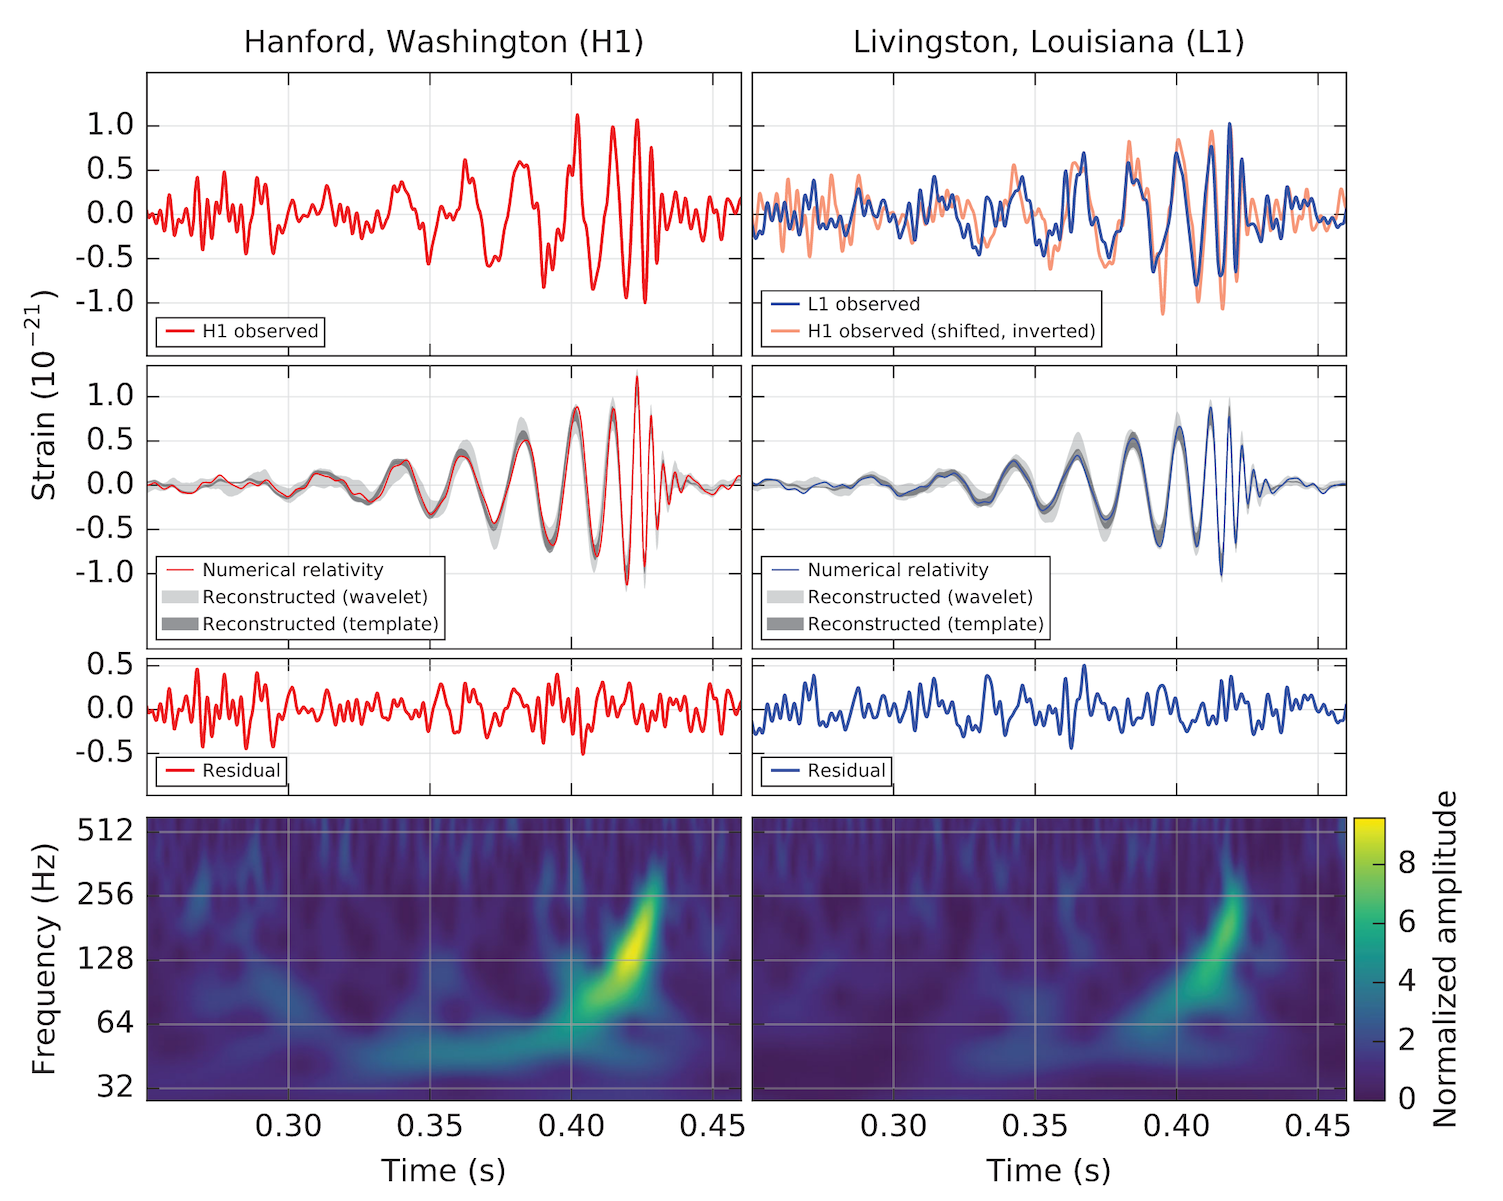
\includegraphics[width=\textwidth]{Assignments/figures/dc_fg.png}
  \end{center}
  \caption{The figure is from: B. P. Abbott et al. (LIGO Scientific Collaboration and Virgo Collaboration)
    Phys. Rev. Lett. 116, 061102 – Published 11 February 2016}
  \label{fig:ligo_result_plot}
\end{figure}


\section{7. Time delay}

Gravitational waves are expected to propagate at the speed of
light. The Hanford and Livingston detectors are separated by about
3000 km. A gravitational wave will propagate this distance in about 10 ms.

The gravitational wave angle of arrival is not known, but the relative
time delay between the signal detected at Hanford and Livingston is
expected to be $-10 < \tau < 10$ ms, if it is moving at the speed of
light in vacuum.
\begin{enumerate}[a)]

  \item Determine the time separation between the two signals \emph{by plotting the magnitudes}
        of the filtered gravitational wave signals ($|y_L[n]|$ and $|y_H[n+n_0]|$) with
        different delays $n_0$ on the same plot. Try different values of $n_0$ until the
        signals are approximately aligned in time. The magnitude of the signal is used to
        avoid phase-time ambiguities. Hint: Use magnitude, not amplitude.
        Magnitude can be obtained using \verb|numpy.abs|.

  \item What value do you obtain for the sample delay $n_0$?

  \item What time delay $\tau$ in seconds does the sample delay $n_0$ correspond to?

  \item Is the time delay $\tau$ in agreement with gravitational-wave
        propagation speed (i.e., that $-10 < \tau < 10$ ms)?

\end{enumerate}

\section{8. Dynamic spectrum}

\begin{marginfigure}
  \begin{center}
    \includegraphics[width=\textwidth]{Assignments/figures/dynspec.png}
  \end{center}
  \caption{A dynamic spectrum plot of the gravitational wave signal.}
  \label{fig:dynspec_ligo_ex}
\end{marginfigure}

Study the time-frequency behavior of the gravitational wave signal.
\begin{enumerate}[a)]

  \item Calculate the dynamic spectrum (spectrogram) of the low-pass
        filtered whitened signal $|\hat{x}[t,k]|$, where $t$ is time and $k$
        is frequency.

  \item Plot the dynamic power spectrum $|\hat{x}[t,k]|^2$ in dB scale.
        Perform this in such a way that you can see the time-frequency response
        behavior of the gravitational wave signal clearly. Plot your result at
        between $t=15.5$ s and $t=17$ s. Hint: You will need to use zero-padding,
        a tapered window, and overlapping windows. An example of the time-frequency
        domain behavior of the gravitational wave signal is shown in Figure \ref{fig:dynspec_ligo_ex}.


\end{enumerate}


\section{9. Extra task}
For earning an extra point, improve any part of the signal processing
in a way that you see fit. Document your improvements. You can, e.g.,
try to create a filter that removes only the strong frequency
components from the signal, or you can use a better low-pass filter.

\begin{figure}
  \begin{center}
    \includegraphics[width=\textwidth]{Assignments/figures/ligo_nobel.jpg}
  \end{center}
  \caption{The gravitational wave measurement using a Michelson-Morley interferometer. Credits: Johan Jarnestad, The Royal Swedish Academy of Sciences.}
  \label{fig:ligo_nobel_diag}
\end{figure}

